\visHeader

Enterprise Architect (EA) is a visual modelling tool that supports UML\footnote{Unified Modelling Language} and a host of other modelling languages.
EA is not only affordable but also quite flexible and can be extended via \emph{extensions} to support new modelling languages.
\begin{itemize}
\item[$\blacktriangleright$] Download EA for Windows from \url{http://www.sparxsystems.com/} to get a free 30 day trial and follow installation instructions (Fig.~\ref{fig_enterpriseArchitextHomepage}).

\begin{figure}[htbp]
	\centering
  	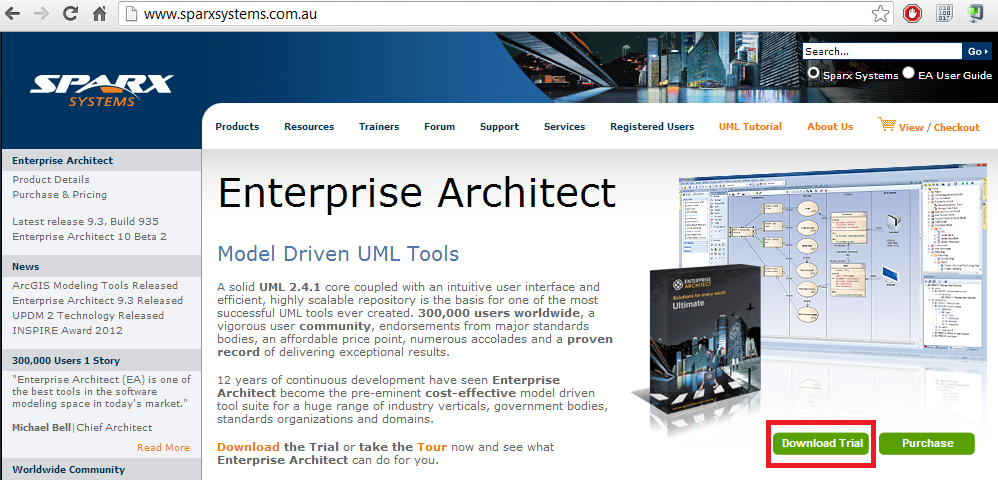
\includegraphics[width=0.77\textwidth]{ea_download}
	\caption{Download Enterprise Architect}
	\label{fig_enterpriseArchitextHomepage}
\end{figure} 

\item[$\blacktriangleright$] Install our EA-Extension (Fig.~\ref{fig_eaPluginWizard}) to add support for our modelling languages.
Download \url{http://www.moflon.org/fileadmin/download/moflon-ide/eclipse-plugin/ea-ecore-addin/ea-ecore-addin.zip}, unpack, and run \texttt{setup.exe}.

\begin{figure}[htbp]
	\centering
  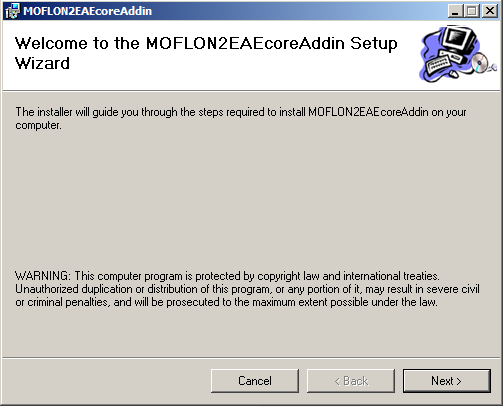
\includegraphics[width=0.55\textwidth]{eaplugin_install}
	\caption{Install our extension for EA}
	\label{fig_eaPluginWizard}
\end{figure}
\end{itemize}